%!TEX root = ../main.tex

\chapter{Background and Related Work}
\label{chapter:overview}
This chapter presents some background on epilepsy and the frequency components present in signals from data recordings in epileptic patients. This is followed by a survey of related works on quantitative analysis techniques on these data for tracking epileptic seizure networks. 

\section{Epilepsy}
The International League Against Epilepsy (ILAE) and the International Bureau for Epilepsy (IBE) have defined epileptic seizure as a transient occurrence of signs and symptoms due to abnormal excessive or synchronous neuronal activity in the brain \citep{fisher2005epileptic}. Such seizures usually induce drastic changes in cognitive processes of an individual. 
The area of the cortex from where the seizure is generated is called \textit{seizure onset zone (SOZ)}. It is also called the epileptic focus or seizure focus. 

The period between the beginning of symptoms in epileptic patients such as consciousness loss or uncontrolled movement to the end of such symptoms is called the ictal state. This can last from a few seconds to few minutes long. These symptoms are accompanied by highly synchronous electrical activities in the SOZ that typically spread to much wider areas of brain. The state immediately prior to the visible seizure onset is called pre-ictal. The interval between two seizures is called inter-ictal and can last from many hours to days or even years. The ictal period is dominated by synchronous electrical activity in the SOZ and areas of spread. The time prior to the seizure is called pre-ictal which can last from seconds to minutes. The experience can be different for different patients. Figure \ref{fig:seizure-onset-sample} shows a sample iEEG recording on a representative patient. The seizure onset electrode in the SOZ is highlighted.

A seizure that begins with a single or localized origin is called a focal or partial seizure. The majority of refractory epileptic patients fall under focal (partial) epilepsy. Surgical resection of the seizure focus remains their best hope for cure. Various imaging modalities are used in combination to get a complete picture of the events or disorder, and to localize the seizure focus.  

\begin{figure*}
\centerline{
	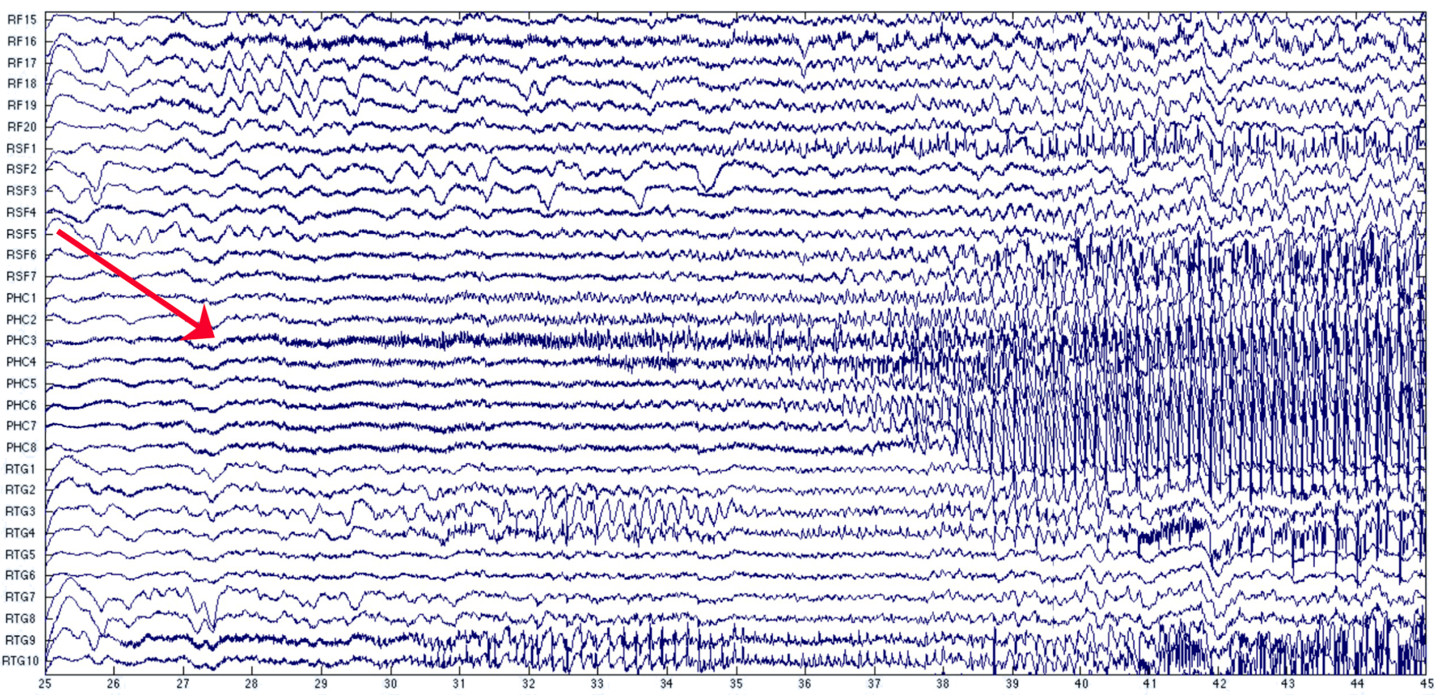
\includegraphics[height =3in]{Plots/Seizure-onset-sample.jpg}
	}
	\caption{IEEG recording of the focal seizure on the representative patient. X-axis represents the time in seconds and y-axis represents the recording sites or electrodes. The arrow shows the electrode contact from where the seizure started. The synchronous activity expanded to other areas in a few seconds.
	\label{fig:seizure-onset-sample}
}
\end{figure*}

\section{Clinical modalities of interest}

\subsection{Intracranial EEG Recording (iEEG)}
Intracranial electroencephalography (iEEG) is a type of invasive electrophysiological monitoring. Most commonly depth electrodes consisting of 1-D linear electrode arrays, shaped in the form of needles, are implanted through cortex into deeper and sub-cortical brain regions. Continuous electrical activities are recorded from these electrodes to capture seizure activities, along with simultaneous video monitoring. Usually, a patient stays in an epilepsy monitoring unit (EMU) for a few days to weeks to record multiple episodes of seizure. The decision for the resection areas are based upon the SOZ identified from these recordings. Figure \ref{fig:structural_scan} shows the positions of implanted depth electrodes in the MRI scan for a representative patient. The red box marks the SOZ as identified from iEEG recording. iEEG provides much better spatial and temporal resolution compared to scalp EEG as these are implanted in the proximity of cortical electrical activity generators. However, the invasiveness of this method can introduce risk of infection, bleeding, strokes and other complications. iEEG can only sample a small area of the brain with a finite number of implanted electrodes. In order to sample the whole brain volume with the present spatial resolution of 3.5mm, about 10,000 recording sites are required \citep{lachaux2003intracranial}. At present, the maximum number of implanted electrodes is a few hundred. Subject to these limitations, there has been growing interest in the combined application of iEEG with non-invasive techniques like functional Magnetic Resonance Imaging (fMRI). 

\begin{figure*}
\centerline{
	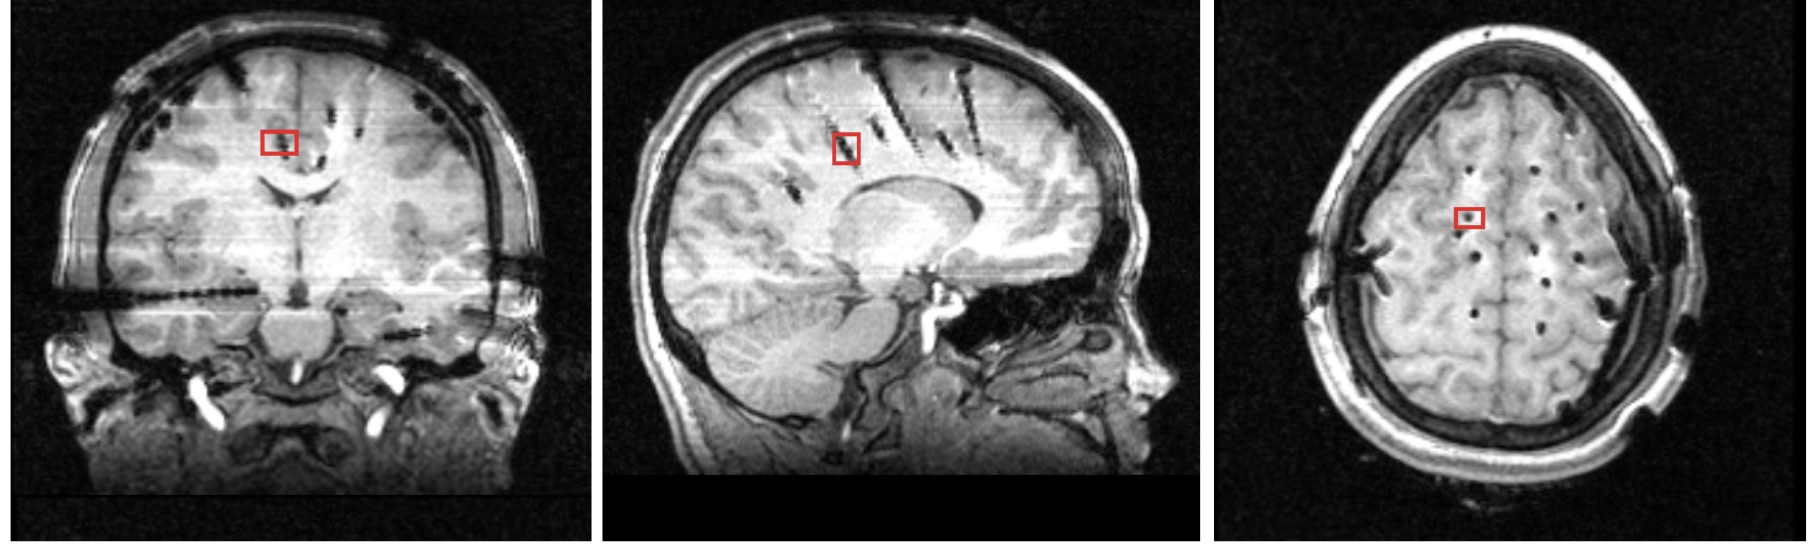
\includegraphics[height =2in]{Plots/Structural scan.jpg}
	}
	\caption{ Magnetic Resonance Imaging (MRI) scan of a patient. An array of electrodes is implanted in the region of the hypothesized SOZ, with 10 contacts for each electrode. The red box highlights the SOZ.
	\label{fig:structural_scan}
}
\end{figure*}


\subsection{Functional Magnetic Resonance Imaging (fMRI)}
Functional Magnetic Resonance Imaging (fMRI) technique is a non-invasive indirect mea- surement of the local neuronal activity which tracks the changes in blood oxygenation over involved brain areas and time. fMRI images are based on the physiological contrast of blood oxygen saturation, thus it is often termed blood-oxygen level dependent (BOLD) signals \citep{ogawa1990oxygenation}. Increased neuronal activity can lead to higher energy demand and vascular changes, which in turn increases the oxygen-rich blood flow and the intensity of recorded BOLD signals \citep{huettel2004functional}. The smallest 3 dimensional smallest unit of these images is called a voxel.

The fMRI signals recorded when the patient is not performing any specific task is called resting state fMRI (rsfMRI). Patients are instructed to lie down with eyes open (or closed), fixated at a screen during collection of fMRI data. The spontaneous low frequency fluctuations ($< 0.1$ Hz) of rsfMRI BOLD signals are utilized to produce surrogate markers for various physiological states and also pathological conditions.

fMRI has been widely used to investigate functional connectivity and large scale network activities in the brain \citep{fox2007spontaneous}. The network between two brain areas or voxels can be studied by a) Seed based correlation maps, b) Spatial independent component analysis of fMRI, or the spatial map of co-varying voxels, and c) Causality analysis between nodes (brain areas) to investigate network dynamics using computation models like dynamic causal models (DCM), structural equation modelling and Granger Causality \citep{centeno2014network}. 

Several research studies have applied these techniques in attempts to localize the SOZ and included prospective patient series, and a few seem rather promising.  However, in general these studies have some pre-defined limitations, identify blobs rather than networks \citep{shah2019characterizing, boerwinkle2017correlating, gil2020beyond, hunyadi2013ica, zhang2015lateralization}, and have not been directly correlated with epilepsy networks as assessed by EEG or other techniques. Fine mapping of spectral (frequency specific) and spatial network from ictal EEG to resting state fMRI could assist in accurate localization of the SOZ, in time and space, further enhancing understanding of the origin and propagation of seizures.
 
\section{Brain oscillations}
iEEG recording consists of frequencies from very low (0.01 Hz) to very high ranges (600 Hz or more). Many studies consider 0.008 Hz to 0.2 Hz as the artifact free useful resting state fMRI BOLD signal \citep{deramus2020modular}. Frequencies higher than 0.2 Hz have been shown to contain useful information in the BOLD signal but can consist of artifacts as well. These broadband frequencies have been observed in different parts of the brain in healthy and neurological conditions. These frequencies are also observed in various task based recordings. 

\subsection{Classical frequencies}
The range from 1 to 80 Hz is sometimes called the classical EEG frequency range, subdivided into frequency bands such as delta (1-3 Hz), theta (4-8 Hz), alpha (8-12 Hz), beta (13-30 Hz, and gamma (30-80 Hz). These classical frequencies have been shown to be associated with different processes like working memory (theta oscillations), alertness, attention and semantic memory (alpha oscillations), cognitive processing (beta oscillations), visual, auditory and motor tasks (gamma oscillations). Few studies have shown coupling of these oscillations with high frequency activities with respect to epilepsy \citep{hashimoto2020coupling, hashimoto2021phase}.

\subsection{High frequency activities}
High frequency oscillations $> 80$ Hz are often subdivided into ripples (80-200 Hz) and fast ripples (200-500 Hz). Two important aspects necessary for recording HFOs are the size of the electrodes and sampling frequency. Recently, commercially available clinical electrodes with specification 4$mm^2$ have been shown to record HFOs in human depth and subdural recording from both temporal and neocortical areas, in both ictal and interictal phases \citep{ochi2007dynamic, worrell2008high, crepon2010mapping, wu2010removing}. The maximum frequency that can be evaluated for HFOs is half of the sampling frequency (Nyquist frequency). Due to the limitations of filters in EEG systems however, the maximum frequency that can be evaluated is about 1/3 of the sampling frequency, requiring at least 240 Hz to record 80 Hz \citep{modur2014high}. HFOs may be generated by inhibitory post-synaptic potentials of the inter-neurons on the pyramidal cells, which are the primary excitation units in human cortex. The fast and synchronous firing of pyramidal cells can be facilitated at a cellular level by neuronal communication methods like axonal sprouting (growth of axons), electrotonic coupling (direct connection between cytosolic contents of adjacent cells), and ephaptic transmission (connection caused by exchange of ions) \citep{jiruska2010electrographic}. HFOs have been associated with both normal and pathologic brain functions. HFOs could play a role in episodic memory and is found to be associated with normal functioning of neocortex. HFOs of hippocampus have been shown to be related to pathologic conditions. Pathologic HFOs have been shown to be helpful in defining epileptic seizure, localizing the SOZ, and identifying propagation pathways in ictal and interictal states \citep{zijlmans2011ictal}. 

\subsection{Infraslow activities}
Infraslow frequencies have been identified variously as - “ultraslow,” “subdelta,” “baseline shifts,” or “near DC” EEG activity in the literature. The upper boundary of recorded activity range from 0.1 Hz \citep{miller2007ictal}, 0.2 Hz \citep{modur2012seizure}, and 0.5 Hz \citep{murai2020scalp} and the lower boundary between 0.01 and DC \citep{kim2009ictal}. In this study, we consider 0.01 to 0.1 Hz as the infra-slow activity (ISA) range. 

There are relatively few studies of ISA in epilepsy. This could be due to past equipment lim- itation of the EEG system with relatively low input impedance and unstable DC baselines over time, and suboptimal electrode/electrolyte interfaces. More recent epilepsy case series argue that widely-available passbands, using conventional EEG systems, are sufficient to provide valuable IsEEG data for visual analysis \citep{rampp2012ictal}. The number of studies is expected to increase with the recent development of wider passbands of the amplifiers, platinum electrodes, and gigaohm input impedances.

The generation of ISA is linked with neuronal and glial activity along with blood brain barrier alteration. The neuronal depolarization during seizure causes an increase in extracellular potassium and glial depolarization. The conduction of this depolarization due to neuron-glial interaction results in negative shifts in deep recording and positive shifts in superficial electrode recordings \citep{shorvon2015treatment}. ISA has been found in many brain regions both in healthy \citep{mitra2015propagated} and pathological conditions \citep{hughes2011infraslow}. 

ISA activities have been observed in qualitative studies before seizure onset \citep{modur2012seizure}, but the quantitative analysis of ISA has been rare. In a recent study by Hashimoto et. al, ripple activities during seizure evolution have been found to be phase amplitude coupled (PAC) with infra-slow (0.016-1Hz) \citep{hashimoto2020coupling} and theta oscillations (4-8 Hz) a few minutes before seizure onset \citep{hashimoto2021phase}. 


%The quantitative analysis of ISA have potential to help in the localization and understanding of seizure origin and propagation.

%None of these studies involved rigorous quantitative analysis of infraslow activity as the basis for a particular choice of frequency range. We applied the main computational tool of this thesis, Granger causal flow, to estimate which portion of this broad range appeared to carry the largest amount of critical information in one subject.

%These preliminary results suggest that the higher frequency ranges suggested by some authors for infraslow might be suboptimal, and further elaboration of our calculations could provide the basis for a more empirical redefinition of the infraslow frequency range.

%Early EEG systems were poorly suited to very low frequency recording, having relatively low input impedance, unstable DC baselines over time, and suboptimal electrode/electrolyte interfaces. Specially designed amplifiers and careful skin preparation were required, but these modifications were feasible only with the relatively small number of channels needed for scalp recording. In the modern era of intracranial EEG recording, where hundreds of contacts and channels may be used, the acquisition of additional special amplifiers in such numbers is financially impractical, and routinely implanting a second set of electrodes virtually impossible. So researchers are practically confined to amplifiers optimized to a higher bandwidth, and to platinum-based electrodes that are biologically inert and compatible with MRI imaging. Manufacturers generally do not provide specifications for the performance of their systems at ISEEG frequencies. However, modern amplifiers generally feature far more stable operation and gigaOhm input impedance.

%Based upon comments from Rampp and Stefan \citep{rampp2012ictal}, and the observation that our own unfiltered EEG data showed very wide variations in DC baselines among different channels (in the range of many millivolts) we used a custom-built ultra low-frequency sine wave generator to directly measure the performance of the Natus amplifiers used for our EEG recordings. Balanced sine wave inputs at wave lengths down to 100 seconds were applied to the inputs. The raw data is shown in Figure \ref{fig:frequency_range}, and the corresponding frequency response curves in Figure \ref{fig:sine-curve-natus-filter-setting}. The colored curves correspond to the Natus filter settings. The X axis displays the frequencies of the input sine waves and the Y axis the measured amplitude of the recorded signal. The three curves to the right, corresponding to digital high pass filter settings of 0.03 - 0.30 Hz, extrapolate to typical single pole high-pass filters with an amplitude rolloff of approximately 10 dB/ decade. The curve corresponding to 0.01 Hz appears to show a milder rolloff. The blue curve, corresponding to the "off" setting of the high pass filter and to the raw data parameters used in all of the analysis for these studies, has an even slower rolloff compared to any conventional analog or digital filter, and may represent simply the inherent limitations of the amplifier outside of its designed performance range. This very slow rolloff and the great interchannel variability of DC baselines support the suspicion that with digital filtering “off,” no conventional high-pass filtering of any kind is being applied to the signal. Above 0.01 Hz amplitude rolloff is less than 10 dB. The high voltages of intracranial ISEEG, measured in hundreds of microvolts, means that this leaves a robust signal for quantitative analysis. However, instrumental phase shift is more difficult to determine.

%\begin{figure*}
%\centerline{
	%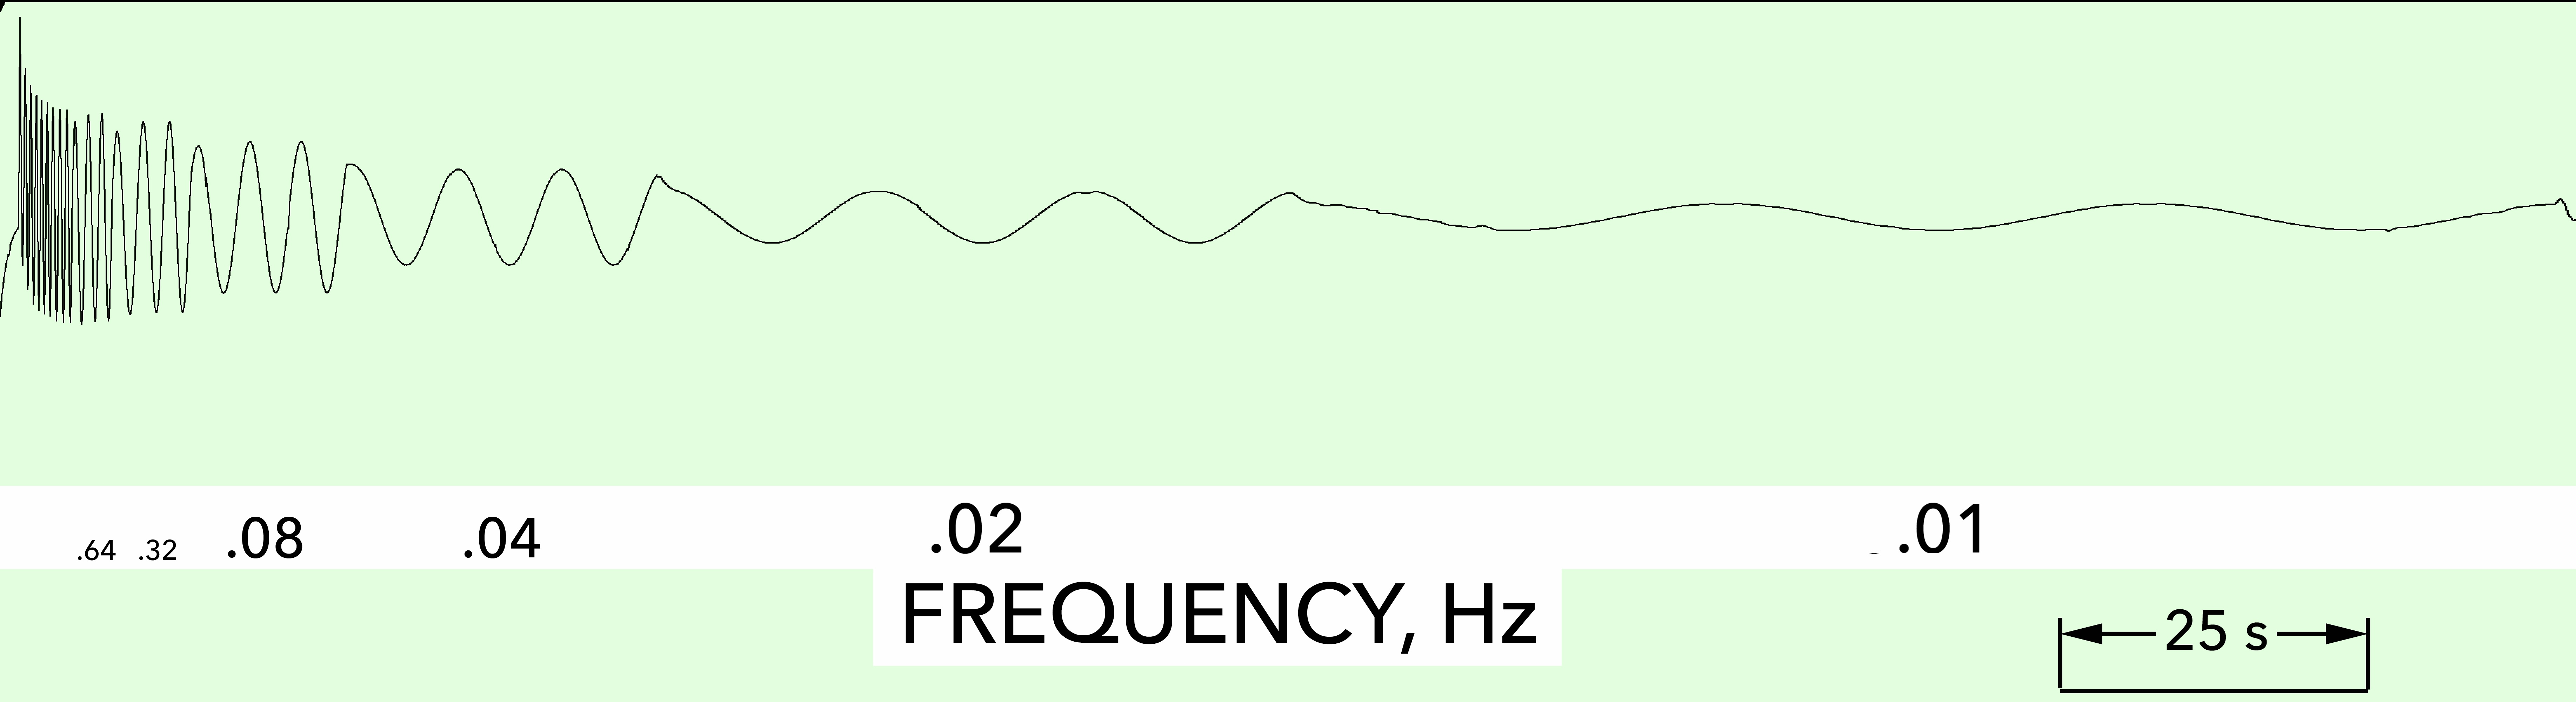
\includegraphics[height %=2in]{Plots/Frequency-range.jpg}
%	}
	%\caption{The full sine wave test curve. Initial offset is due to the custom signal generator, not the recording system 
%	\label{fig:frequency_range}
%}
%\end{figure*}


%\begin{figure*}
%\centerline{
%	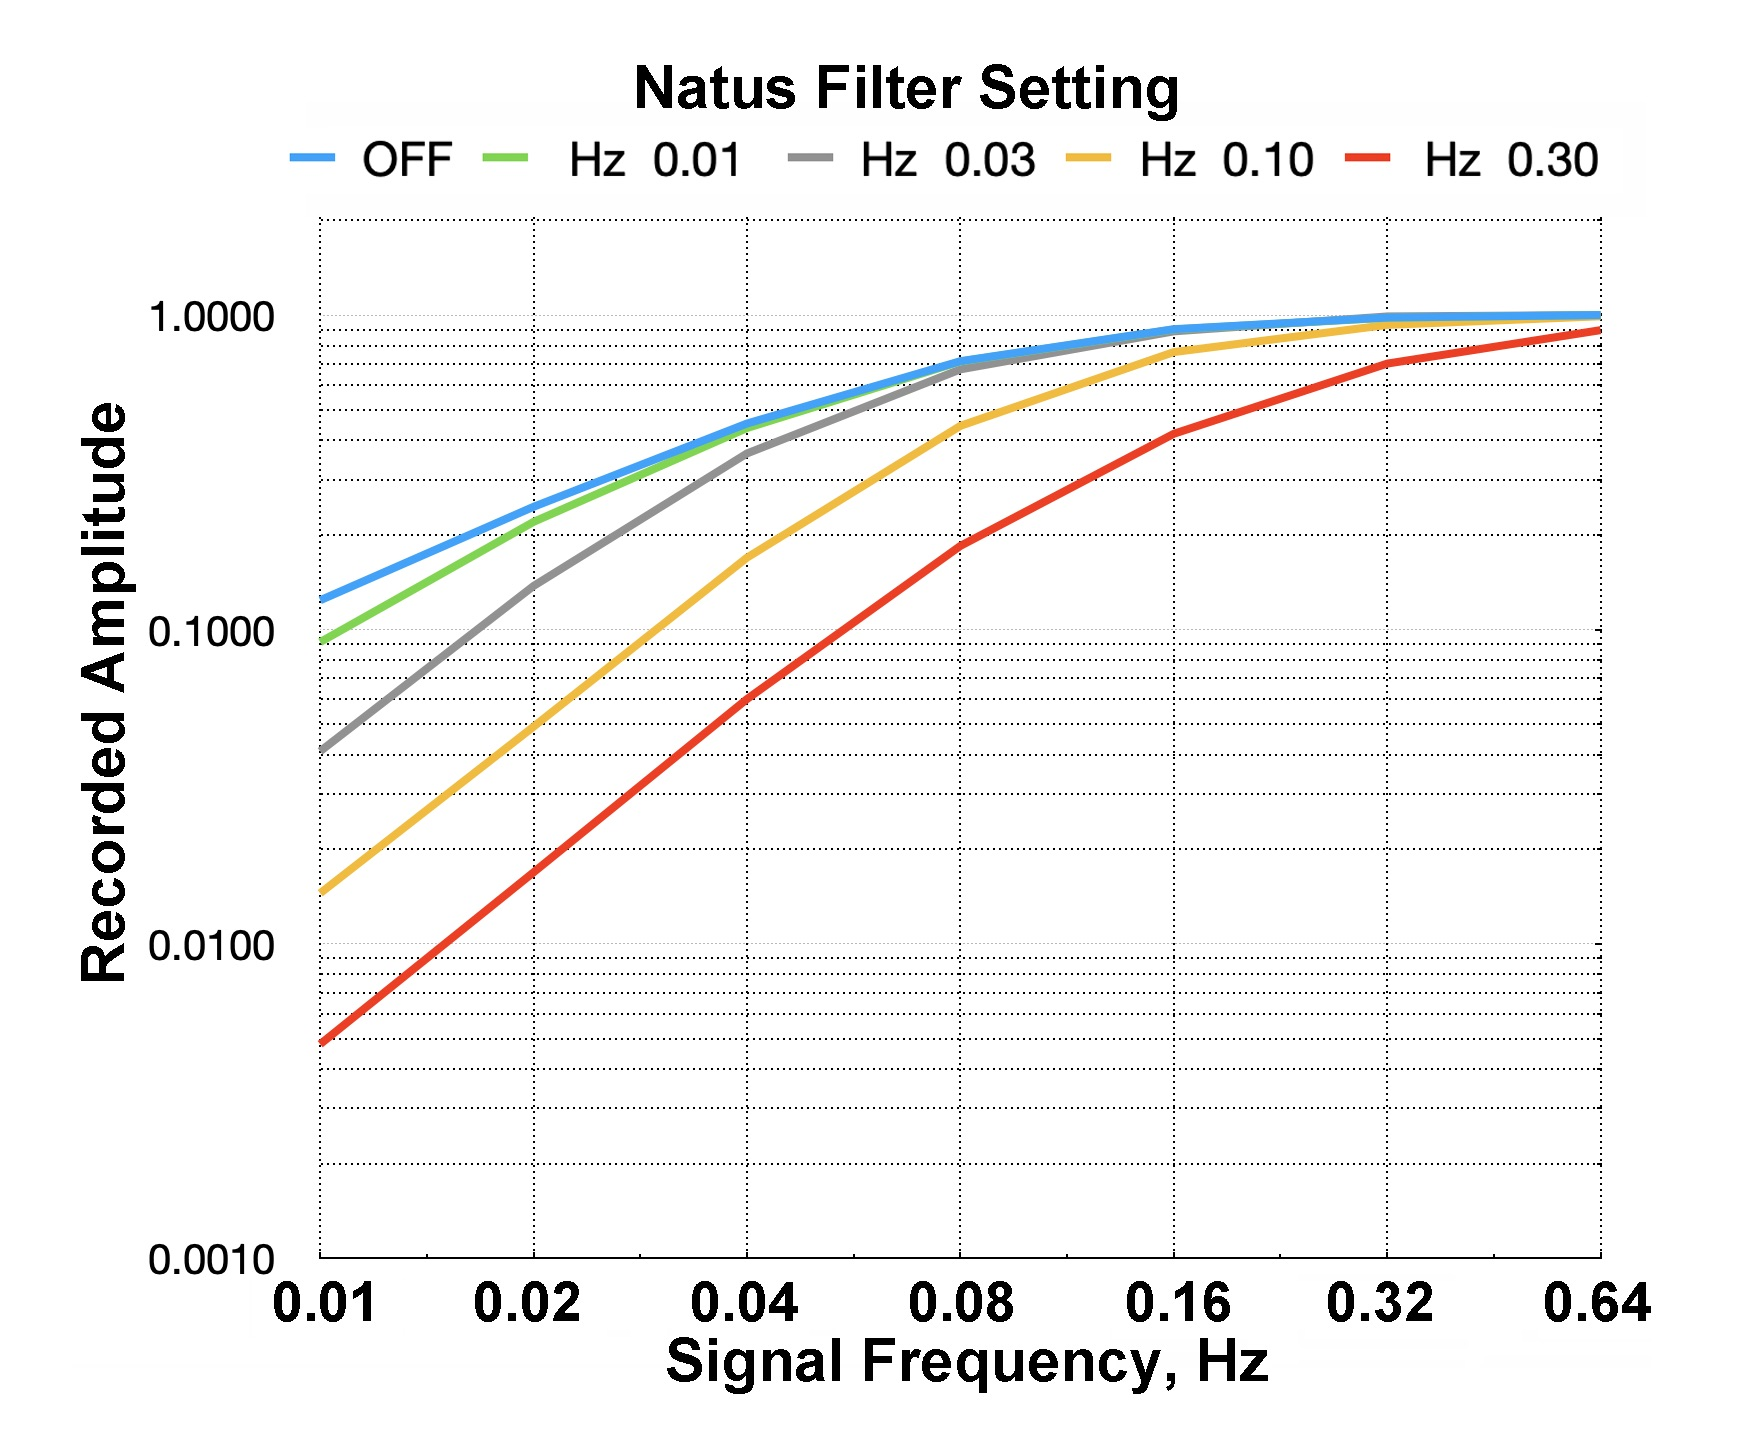
\includegraphics[height %=4in]{Plots/Natus-filter-setting.jpg}
%	}
%	\caption{Frequency response curves derived from the data in Figure \ref{fig:frequency_range}
%	\label{fig:sine-curve-natus-filter-setting}
%}
%\end{figure*}

\section{Quantitative analysis}
Quantitative analysis has been applied to human EEG for well over half a century \citep{grass1938fourier} long preceding the introduction of modern computerized techniques. The study of infra-slow EEG is only a few decades behind \citep{aladjalova1957infra}. However, the early and sustained attention of quantitative studies have been towards higher frequencies rather than the lower. This gap in progression may be due to the technical constraints on the infra-slow recording at the scalp and the arrhythmic nature of the infra-slow EEG as described above. Prior researchers may have assumed that data of this sort was unlikely to carry useful information – especially information that could be extracted by more advanced quantitative techniques.

Recently, there has been an increasing acceptance that a set of distributed regions forms a network during seizure rather than a single focus, thus the recent researchers have applied advanced quantitative methods to model such a system. Many approaches are based on the quantification of the seizure onset zone using a time-frequency analysis of iEEG. 

%Here we review few recent quantitative methods and their application to infra-slow activities, if any.

The linear relationship between iEEG time-series have been estimated using multivariate auto-regressive (MVAR) models in methods like coherence, Granger Causality, direct directed transfer function (dDTF) and partial directed coherence (PDC). The study by \citep{joshi2016regional} have shown strong coherence between electrodes pair 0-2 $cm$  apart in the infra-slow frequency range of ($<0.15 Hz$), but decreased sharply for greater inter-contact distance. DTF methods have been described by \citep{franaszczuk1998application} to determine patterns of flow of activity in pre-ictal periods, whereas \citep{wilke2011graph} discussed the betweenness based on DTF in the classical frequency range for ictal and interictal dataset. \citep{zhang2020establishing} studied graph network derived on partial directed coherence in classical frequency range in both pre-ictal and inter-ictal periods.

\subsection{Granger causality}
Granger causality (GC) is one of the most commonly used methods for determining causal influences (or directional functional connectivity) between dynamical systems by the analysis of their time series measurements \citep{granger1969investigating}. GC is based on the idea of linear prediction by using multivariate autoregressive (MVAR) modeling \citep{wiener1956theory} and uses predictability and statistical dependencies to establish causal relations. GC can be estimated using either autoregressive modeling (parametric methods) or by using direct Fourier or wavelet transforms (non-parametric) spectral decomposition approaches \citep{dhamala2008estimating}, \citep{ding200617}. The definitions and calculation of GC are provided in Appendix \ref{chapter:appendix-definitions}.

Several studies, including from our lab, have successfully utilized Granger causality methods for analysis of high density EEG source waveforms, ICs (independent component) of scalp EEG recording, high frequency activities in preictal, and classical frequencies in in- terictal iEEG \citep{coben2015neural, coito2015dynamic, epstein2014application, park2018granger}. 

\subsection{Graph theory}
A graph is a mathematical structure used to model relations between objects. A graph consists of nodes (vertices) and edges (connection between nodes). Graph theory is the study of graphs (networks), and has been extensively used in numerous studies and applications, including epilogenetic brain network. A graph can be directed, which contains ordered pair of nodes, or undirected, that consists of edges with no specific direction or order. Several graph metrics have been formulated to quantify network characteristics and are widely used in network studies. Some of the commonly used graph measures are Degree and Betweenness. Short descriptions of these measures along with their mathematical definitions are provided in Appendix \ref{chapter:appendix-definitions}.

%Complex dynamical network could be constructed based on the pairwise interactions of iEEG time-series.
Graph theory based techniques have gained interest in the recent years to model the epileptic brain network and find important bio-markers of brain function and dysfunctions. The pairwise interactions of iEEG time-series can be modeled as a graph. Quite a few studies have utilized this method in iEEG signals in preictal, interictal and ictal periods of epilepsy \citep{wilke2011graph, van2013ictal, bartolomei2013interictal, vecchio2016pre}, but none of these include quantitative analysis of infra-slow activities.

\section{Discussion}
Several of the prior qualitative studies and quite a few quantitative studies on infra-slow iEEG have shown promising results for the usefulness of these signals in extracting important biomarkers in an epileptic network. However, to the best of our knowledge, there is no comprehensive study that quantifies the infraslow network and examines its correlation with high frequency activities throughout all stages of focal epilepsy. Chapter \ref{chapter:ieeg-infraslow-hfo-correlation} of this dissertation presents such study where we examine the correlation between the two dfferent frequency ranges throughout all epilepsy stages.
One of the other unexplored areas is the concordance between infraslow iEEG and resting state fMRI and if are able to seed epilepsy network from iEEG to rsfMRI for finer focus localization, which is discussed in Chapter \ref{chapter-seeding-iEEG-to-fmri}.